\begin{figure}[h]
\centering
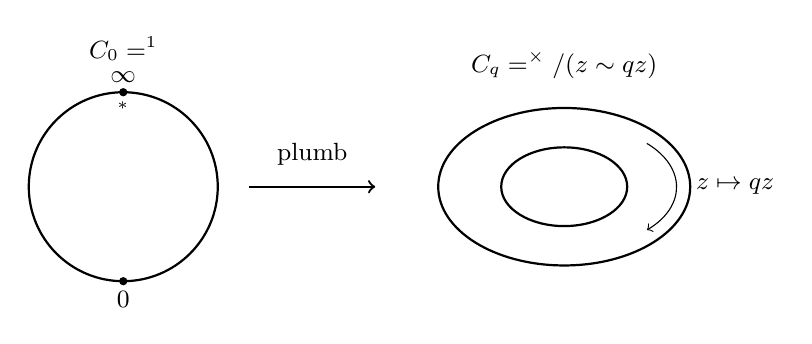
\begin{tikzpicture}[scale=1, every node/.style={font=\small}]
  % C0 = CP^1 with 0 and infinity
  \draw[thick] (-3,0) circle (1.2);
  \node at (-3,1.75) {$C_0=\bbC\bbP^1$};
  \fill (-3,-1.2) circle (1.5pt);
  \fill (-3,1.2) circle (1.5pt);
  \node[below] at (-3,-1.2) {$0$};
  \node[above] at (-3,1.2) {$\infty$};
  \node[above] at (-3,-1.2) {$\vrep$};
  \node[below] at (-3,1.2) {$\vrep^*$};

  % arrow to torus
  \draw[->, thick] (-1.4,0) -- (0.2,0);
  \node[above] at (-0.6,0.15) {plumb};

  % Torus C_q = C^x/(z~qz)
  \begin{scope}[shift={(2.6,0)}]
    % draw a torus-like shape (annulus with identification)
    \draw[thick] (0,0) ellipse (1.6 and 1.0);
    \draw[thick] (0,0) ellipse (0.8 and 0.5);
    \node at (0,1.55) {$C_q=\bbC^\times/(z\sim qz)$};
    \draw[->] (1.05,0.55) .. controls (1.55,0.25) and (1.55,-0.25) .. (1.05,-0.55);
    \node[right] at (1.55,0) {$z\mapsto qz$};
  \end{scope}
\end{tikzpicture}
\caption{Plumbing the punctures on $\bbC\bbP^1$ produces the torus $C_q$.}
\end{figure}
